\section{System Overview}

Our system is designed for exploring and discovering common movement patterns and detecting abnormal situations using LBSN data. The system consists of four major components: a trajectory extraction module, a data analysis module, a context extraction module, and a visualization module as illustrated in Figure~\ref{fig:process}.
%Users first apply a spatiotemporal filter of interest into the system.
%Users select an area and a target time window of interest or a real time mode.
%The users then specify one or multiple past time windows representing normal situations compared to the target time frame.
%We assume that the additional time frames represent normal situations.
The \textit{trajectory extraction module} (Section~\ref{sec:trajectory_extraction}) generates two different sets of trajectories: target and normal trajectories.
%with geo-location information extracted from tweets and Instagram data filtered by the sptiotemporal filter.
The \textit{data analysis module} (Section~\ref{sec:analysis_models}) consists of two components: common movement discovery and abnormal pattern detection. 
For the given trajectory sets, the first component discovers major common routes based on the partition-based clustering model, and the other component assesses the abnormality for each common route.
%More details will be described in Section~\ref{sec:analysis_models}.
\begin{figure}[hbt]
\centering
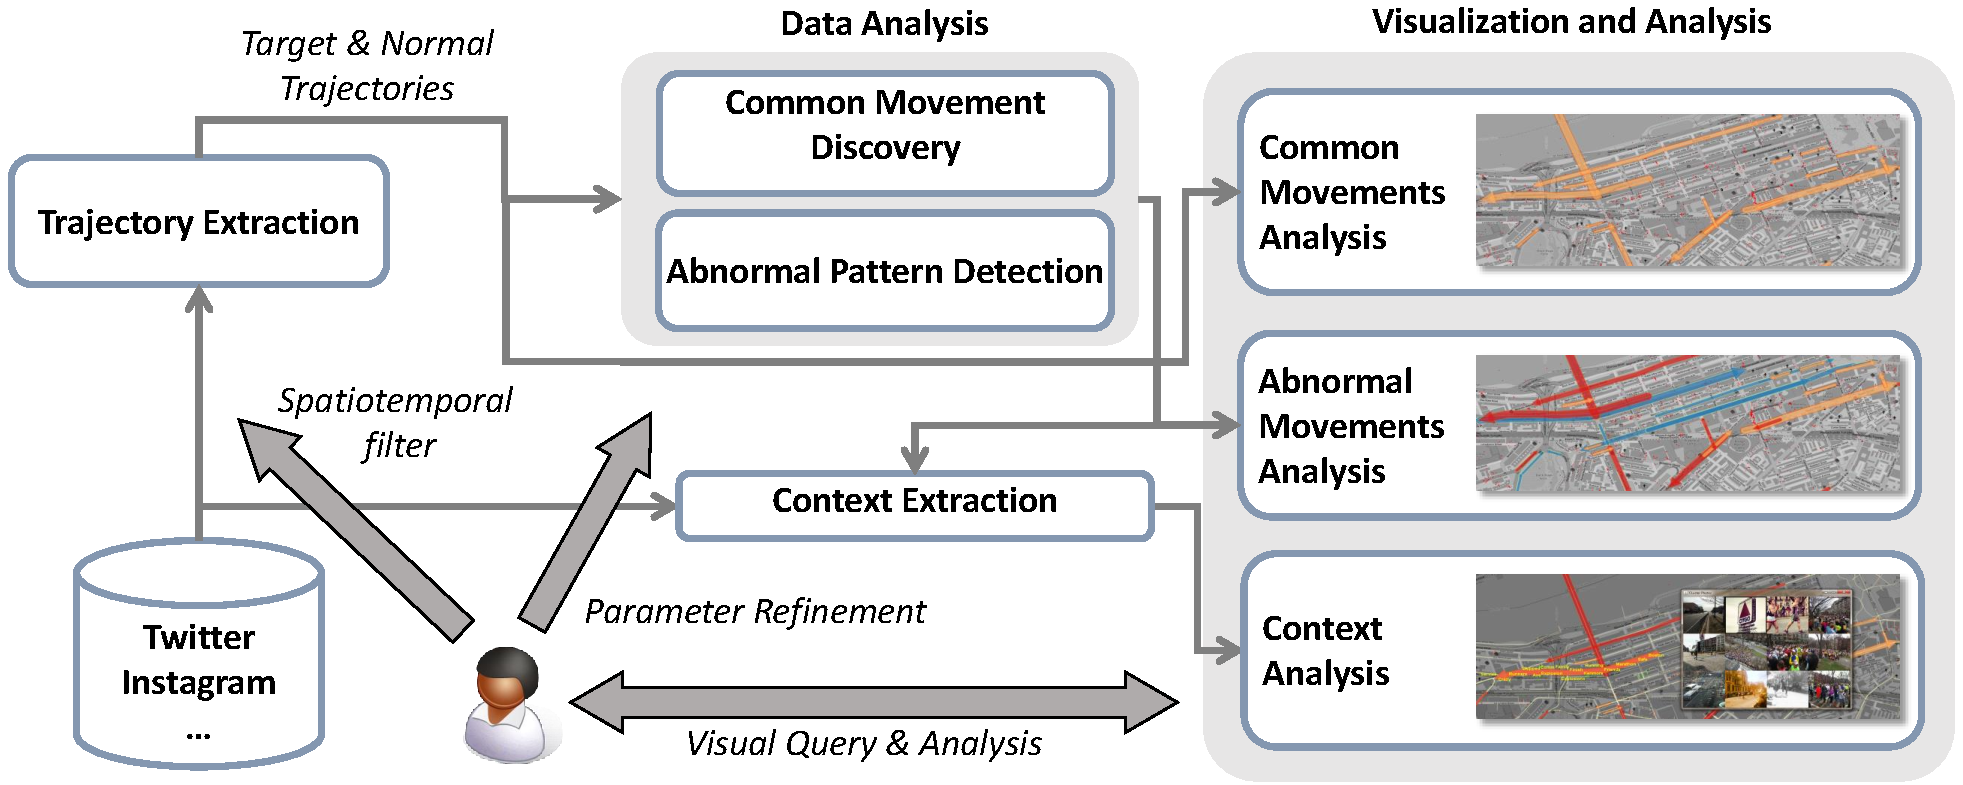
\includegraphics[width=1.0\linewidth]{process_v3}
\caption{Overview of our iterative analysis scheme for human common movement discovery and anomaly analysis.}
\label{fig:process}
%\vspace{-0.4cm}
\end{figure}
The \textit{context extraction module} (Section~\ref{sec:context}) finds relevant context information including keywords, photos, videos from web cameras, and news media based on the results from the analysis module.
The \textit{visualization module} (Section~\ref{sec:visualization}) allows the users to explore the trajectories, common routes, and abnormal movements, and obtain a better understanding of movement patterns using additional context.
Users can iteratively make visual queries and refine the parameters used for clustering and anomaly detection to optimize the results.